
\begin{frame}{Mediciones con el perfilador}

        Calibración del instrumento, medición del colimador F280FC del SPIM
        \begin{columns}[t]
            \begin{column}{0.5\textwidth}
                \begin{figure}[H]
                \centering
                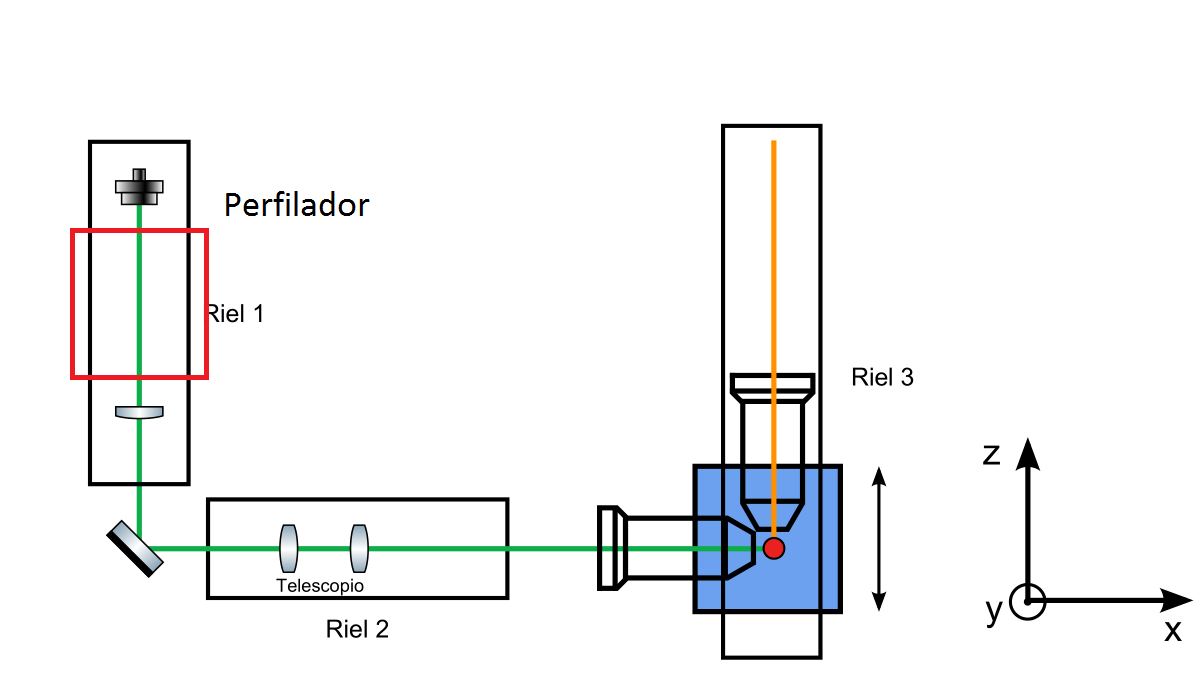
\includegraphics[width=\textwidth]{fig/perfilador/spim_riel_perfilador.png}
                \label{fig:spim_riel_perfilador}
                \end{figure}
                
                 \begin{itemize}
                    \item Inicio del riel:\\ $\sigma = (3,03 \pm 0,15)\,\text{mm}$
                \end{itemize}
                
            \end{column}

            \begin{column}{0.5\textwidth}
                \vspace{-2em}
                \begin{figure}[H]
                    \centering
                    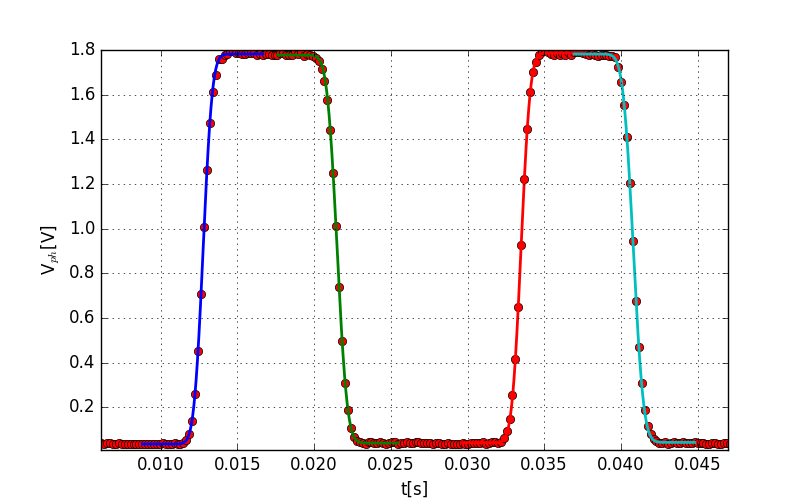
\includegraphics[width=\textwidth]{fig/perfilador/spim_foco_zoom.png}
                    \label{fig:spim_foco_zoom}
                \end{figure}
                \vspace{1em}
                \begin{itemize}
                    \item Fin del riel:\\ $\sigma = (3,02 \pm 0,18)\,\text{mm}$
                \end{itemize}
                
            \end{column}
            
        \end{columns}
        
\end{frame}
    
    \begin{frame}{Medición manual del colimador del SPIM}
            \begin{figure}[H]
                \centering
                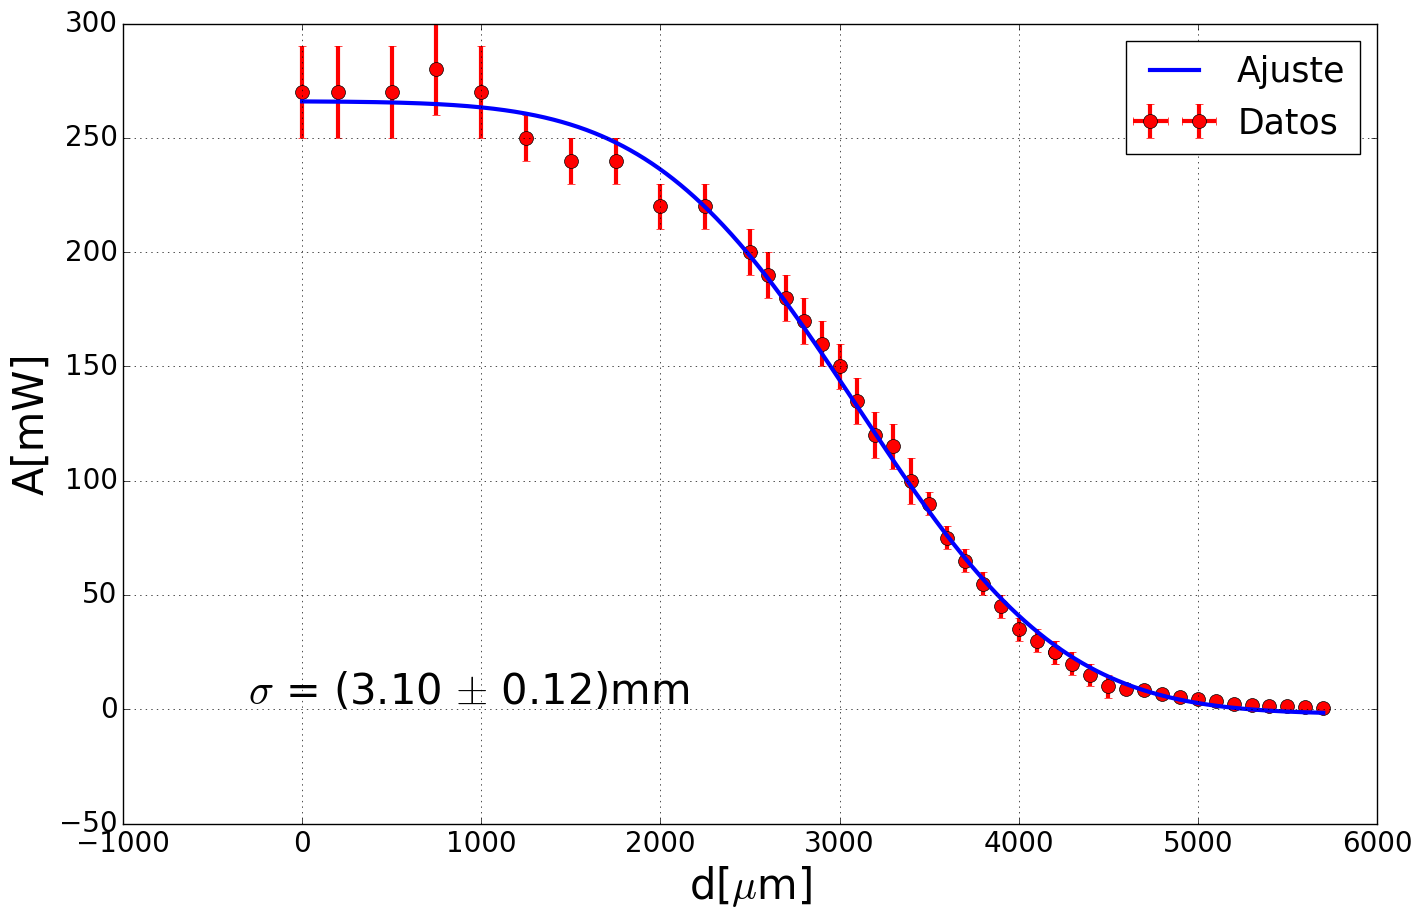
\includegraphics[width=0.7\textwidth]{fig/perfilador/calibracion_f280.png}
                \label{fig:perfilador/calibracion_f280}
            \end{figure}
    \end{frame}

    \begin{frame}{Medición en el telescopio del SPIM}
       \begin{columns}[c]
        \begin{column}{0.5\textwidth}
            \begin{figure}[H]
                \centering
                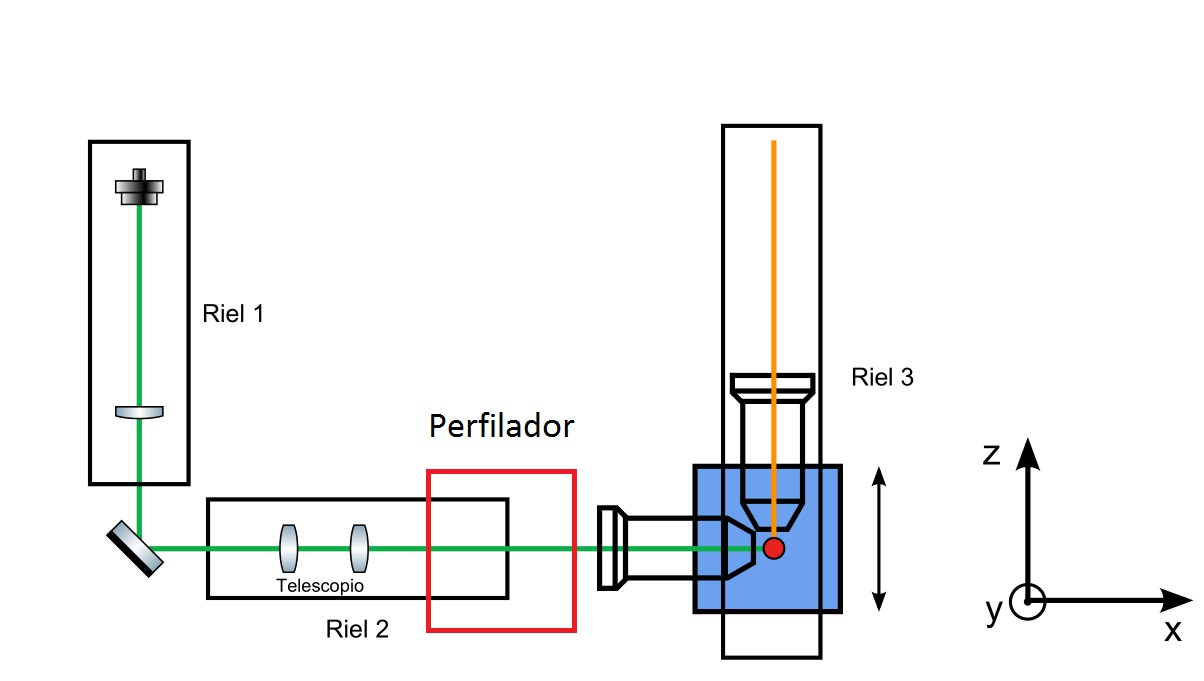
\includegraphics[width=\textwidth]{fig/perfilador/spim_lightsheet_perfilador}
                \label{fig:spim_lightsheet_perfilador}
            \end{figure}
        \end{column}
        \begin{column}{0.5\textwidth}
            \vspace{-3em}
            \begin{figure}[H]
                \centering
                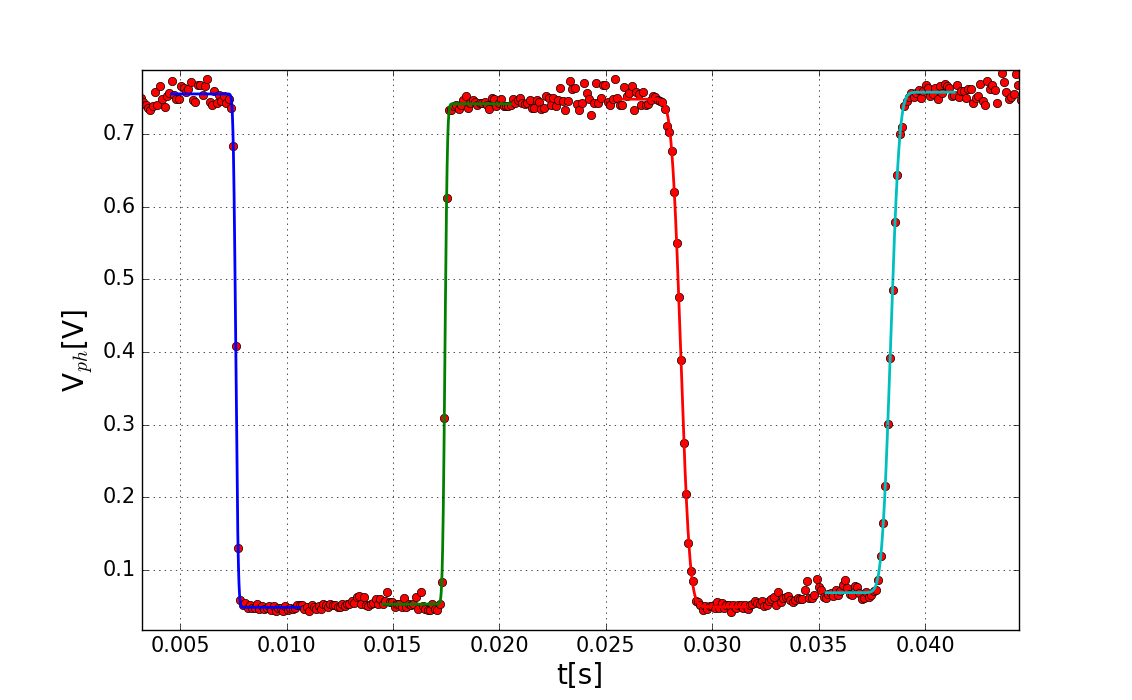
\includegraphics[width=\textwidth]{fig/perfilador/spim_lightsheet}
                \label{fig:spim_lightsheet}
            \end{figure}
            \vspace{-1em}
            Medición a \\d$\approx$80$\,$mm del fin del telescopio
            $\sigma_1 = (0,55 \pm 0,02)\,\text{mm}$\\
            $\sigma_2 = (2,11 \pm 0,05)\,\text{mm}$\\
            \end{column}
        \end{columns}
        \vspace{1em}
        %Las transiciones acusan una \underline{divergencia} apreciable, como es de esperar en un telescopio.

    \end{frame}
